
\documentclass[sigconf]{acmart}
\settopmatter{printacmref=false}


\AtBeginDocument{%
  \providecommand\BibTeX{{%
    \normalfont B\kern-0.5em{\scshape i\kern-0.25em b}\kern-0.8em\TeX}}}




\begin{document}

\title{Development of a blockchain based browser extension for the management of open source repositories on GitHub.}

\author{Michael Frank}
\email{michael.frank@stud.hs-flensburg.de}
\affiliation{%
  \institution{Hochschule Flensburg}
  \streetaddress{Kanzleistraße 91–93}
  \city{Flensburg}
  \state{Schleswig-Holstein}
  \country{Deutschland}
  \postcode{24943}
}

\author{Nico Hohm}
\email{nico.hohm@stud.hs-flensburg.de}
\affiliation{%
  \institution{Hochschule Flensburg}
  \streetaddress{Kanzleistraße 91–93}
  \city{Flensburg}
  \state{Schleswig-Holstein}
  \country{Deutschland}
  \postcode{24943}
}

%%
%% The abstract is a short summary of the work to be presented in the
%% article.
\begin{abstract}
With the development of new technologies such as blockchain, new possibilities are available for the organization of open source projects.In this paper, we present a blockchain-based chrome browser extension for the governance of open source projects on the GitHub platform. This browser extension has an underlying protocol that is intended to decentralize and democratize governance and also provide a financial incentive for participation in open source projects.
\end{abstract}

%%
%% The code below is generated by the tool at http://dl.acm.org/ccs.cfm.
%% Please copy and paste the code instead of the example below.
%%
\begin{CCSXML}
<ccs2012>
 <concept>
  <concept_id>10010520.10010553.10010562</concept_id>
  <concept_desc>Computer systems organization~Embedded systems</concept_desc>
  <concept_significance>500</concept_significance>
 </concept>
 <concept>
  <concept_id>10010520.10010575.10010755</concept_id>
  <concept_desc>Computer systems organization~Redundancy</concept_desc>
  <concept_significance>300</concept_significance>
 </concept>
 <concept>
  <concept_id>10010520.10010553.10010554</concept_id>
  <concept_desc>Computer systems organization~Robotics</concept_desc>
  <concept_significance>100</concept_significance>
 </concept>
 <concept>
  <concept_id>10003033.10003083.10003095</concept_id>
  <concept_desc>Networks~Network reliability</concept_desc>
  <concept_significance>100</concept_significance>
 </concept>
</ccs2012>
\end{CCSXML}

%%
%% Keywords. The author(s) should pick words that accurately describe
%% the work being presented. Separate the keywords with commas.
\keywords{Open source development, Open source, Software development, Development initiative,
		Browser extension, Chrome extension, GitHub, Blockchain, Ethereum, Smart contracts}

%%
%% This command processes the author and affiliation and title
%% information and builds the first part of the formatted document.
\maketitle
\pagestyle{plain}


\section{Introduction}
\subsection{Open source development on GitHub}
Open source development is a type of software development in which a decentralised and collaborative 
community develops software publicly and transparently. Open source development enables the creation 
of innovative and free software through the collaboration of many people, and it also provides free access 
to the software for everyone \cite{shaikh2017governing, redhat2021ops}. Some examples for such significant 
projects are the Linux Kernel \cite{linux2021ops} and the Mozilla Firefox browser \cite{mozilla2021ops}, which are 
used by many people  every day. A particular difficulty in open source development is the coordination of the many 
developers who contribute to the development of the projects with their own extensions or improvements. Changes have 
to be tracked, traced and, if necessary, reversed \cite{shaikh2017governing}. These problems occur not only in open 
source development, but also in normal software development. As in normal software development, version control is 
used to solve these problems \cite{shaikh2017governing, ulrich2020dev}. \\ \\
In particular, the version control protocol Git 
is ideally for open source development, because with Git it is possible to have several distributed remotes that can 
access and manage the same source code \cite{git2021scm, ulrich2020dev}. Projects that are coordinated via git are 
called repositories. The developers have a local copy of the repository on their systems and can push their changes to or 
pull the current status from the main repository. These actions are coordinated via a so-called git server, which has to be 
hosted somewhere so that the developers can work with it \cite{git2021scm}. It is important that this server is permanently 
accessible, otherwise the actions mentioned will no longer work. and coordination of the repository will be 
interrupted \cite{ulrich2020dev}. Hosting services such as GitHub were created so that such problems can be prevented 
and not everyone has to set up their own git server if they want to start an open source project \cite{ulrich2020dev, git2021hub}.
GitHub is the largest git hosting provider today, with over 56 million registered developers and over 100 million repositories.
\cite{git2021hub} The service is also used by large IT corporations such as Microsoft, Facebook and Google and hosts a large 
number of the largest and most important open source repositories \cite{git2021stars}.\\ \\
Normally, an open source project on GitHub starts with a user creating a repository for it. The user who created the 
repository is the owner of it. This user has full control over the repository and can push changes, decide which changes are 
accepted (merged) and even delete the repository. In addition, he can add so-called collaborators to the repository, who have 
read and write rights in the repository \cite{git2021rights}. Normal users who do not have collaboration rights can contribute to 
the open source project by creating a pull request with their change. Another user with the necessary rights can then decide 
whether the change is useful or not. Depending on his decision, he can merge (accept) or reject (reject) the changes. 
The described process is the typical approach to how the community develops for an open source project.


\subsection{Problem}
The described workflow for managing repositories on GitHub but also on other hosting services such as GitLab or Bitbucket has 
some significant disadvantages. Firstly this approach is not necessarily decentralised or democratic. Very few people usually have 
the necessary rights to merge pull requests, and they can decide over the head of the general community whether to merge or reject
 a pull request. So it doesn't matter what the general community thinks, as long as the administrators have a different opinion. Rejecting
 good or useful pull requests is bad, but not a direct threat to the project. The opposite is to merge a critical bug into the main repository,
 which can cause enormous damage, as in the example of the Heartbleed bug in the Open SSL repository \cite{ioriheartbleed}. This 
danger exists mainly because it only takes one person with the necessary rights to overlook the bug and decide to merge the flawed 
pull request. Less critical problems, which nevertheless complicate the work in the communities of open source projects, are the lack
 of initiative for developers to review pull requests or to create pull requests themselves. If an open source repository is not financially
 supported by a company or a large community, they usually live on developers who work on these projects in their spare time, which 
means that further development sometimes takes a very long time. 


\subsection{Solution}
To solve these problems, this paper presents the development of a chrome browser extension that uses the GitHub API  \cite{git2021api} and 
smart contracts \cite{eth2021contracts} on the Ethereum blockchain \cite{eth2021doc} to enable decentralised management of pull requests in GitHub repositories with a 
financial incentive for the community. Using the Ethereum Blockchain, the community can vote on which pull requests should be 
merged or rejected, with decisions to merge good requests and reject bad ones being rewarded. In addition, the community can 
use a crowdfunding mechanism to pool Ether, the native currency of the Ethereum blockchain, to pay developers for solving problems 
or bugs. The functioning of the protocol on which the browser extension is based is explained in detail in \textit{3. Protocol}. Our goal with
 this browser extension and this paper is to solve the problems mentioned and to improve the way open source development 
is done. (Hier Crpytowirtschafts und spieletheorie rein).

\section{Related work}
Related work falls into three areas: \textit{repository governance}, \textit{decentralised voting} and \textit{developer initiative}. 
Previous work has already looked at decentralised approaches to manage GitHub repositories. One work pursues the idea that 
a repository always belongs to the ownerless protocol and that pull requests can only be merged or rejected by the community 
via this protocol. This should prevent the danger that users with writing rights misuse them \cite{ulrich2020dev}. \\ \\
Furthermore trustless and decentralised voting on the blockchain is a topic that has been addressed in several papers 
and which also plays a critical role in this paper \cite{khoury2018decentralized, ulrich2020dev}. \\ \\
In addition, the lack of financial incentive to implement problems or changes in a repository is an issue that has been investigated. 
The research looked at what is important to the developer who solves the bounty and what is important to the financial backer of 
the bounty. \cite{zhou2019bounties}

\section{Protocol}
The described browser extension basically consists of two parts. A frontend that allows users to vote on pull requests or to back 
a bounty financially, and a kind of protocol that runs locally in the browser extension but uses the GitHub API and the Ethereum 
blockchain to take over actions such as distributing stakes or merging and rejecting pull requests by the vote outcome.
The protocol is the actual solution how the control of the pull request management is decentralised, the frontend on the 
other hand provides the possibility to interact with the protocol. In the process of development and research, a total of two 
protocols were designed, with the second protocol being an extension of the first. Adding further functionalities that we 
subsequently deemed as important. This section introduces both protocols and their differences on a non to technical level.

\subsection{First protocol}
The first protocol starts with a developer deciding to develop a change and creating a pull request so that it can be merged into the 
main branch of the repository. After the pull request has been created, any community member, i.e. anyone who follows the repository, 
can start the voting phase for the pull request. In this step, a smart contract is created which is used for the later voting and the distribution
 of the stakes.The community can then vote for or against the pull request for a certain period of time.
When someone submits a vote, they must weight it with a stake. Ether is used as a stake and the more Ether is staked on a vote, 
the higher its weight of it. After the voting period has expired, the protocol adds up the stakes for and against the pull request. \\ \\
If the majority of the stakes, i.e. more than 50 percent, have staked for the pull request, it is merged, otherwise it is rejected.
It is important to note that stakes votes cannot be changed subsequently, once the stake has been sent to the smart contract, 
it is held until the vote is resolved.  After that, the majority stakers divide the stakes of the minority stakers among themselves. 
They get a percentage share of the minority stakes in relation to their stakes in the winning pool. A staker whose decision has won
 and who represents 50 percent of the majority stakes receives half of the minority stakes. The complete process is graphically 
illustrated in \textit{Figure 1}.

\begin{figure*}[h]
	\centering
	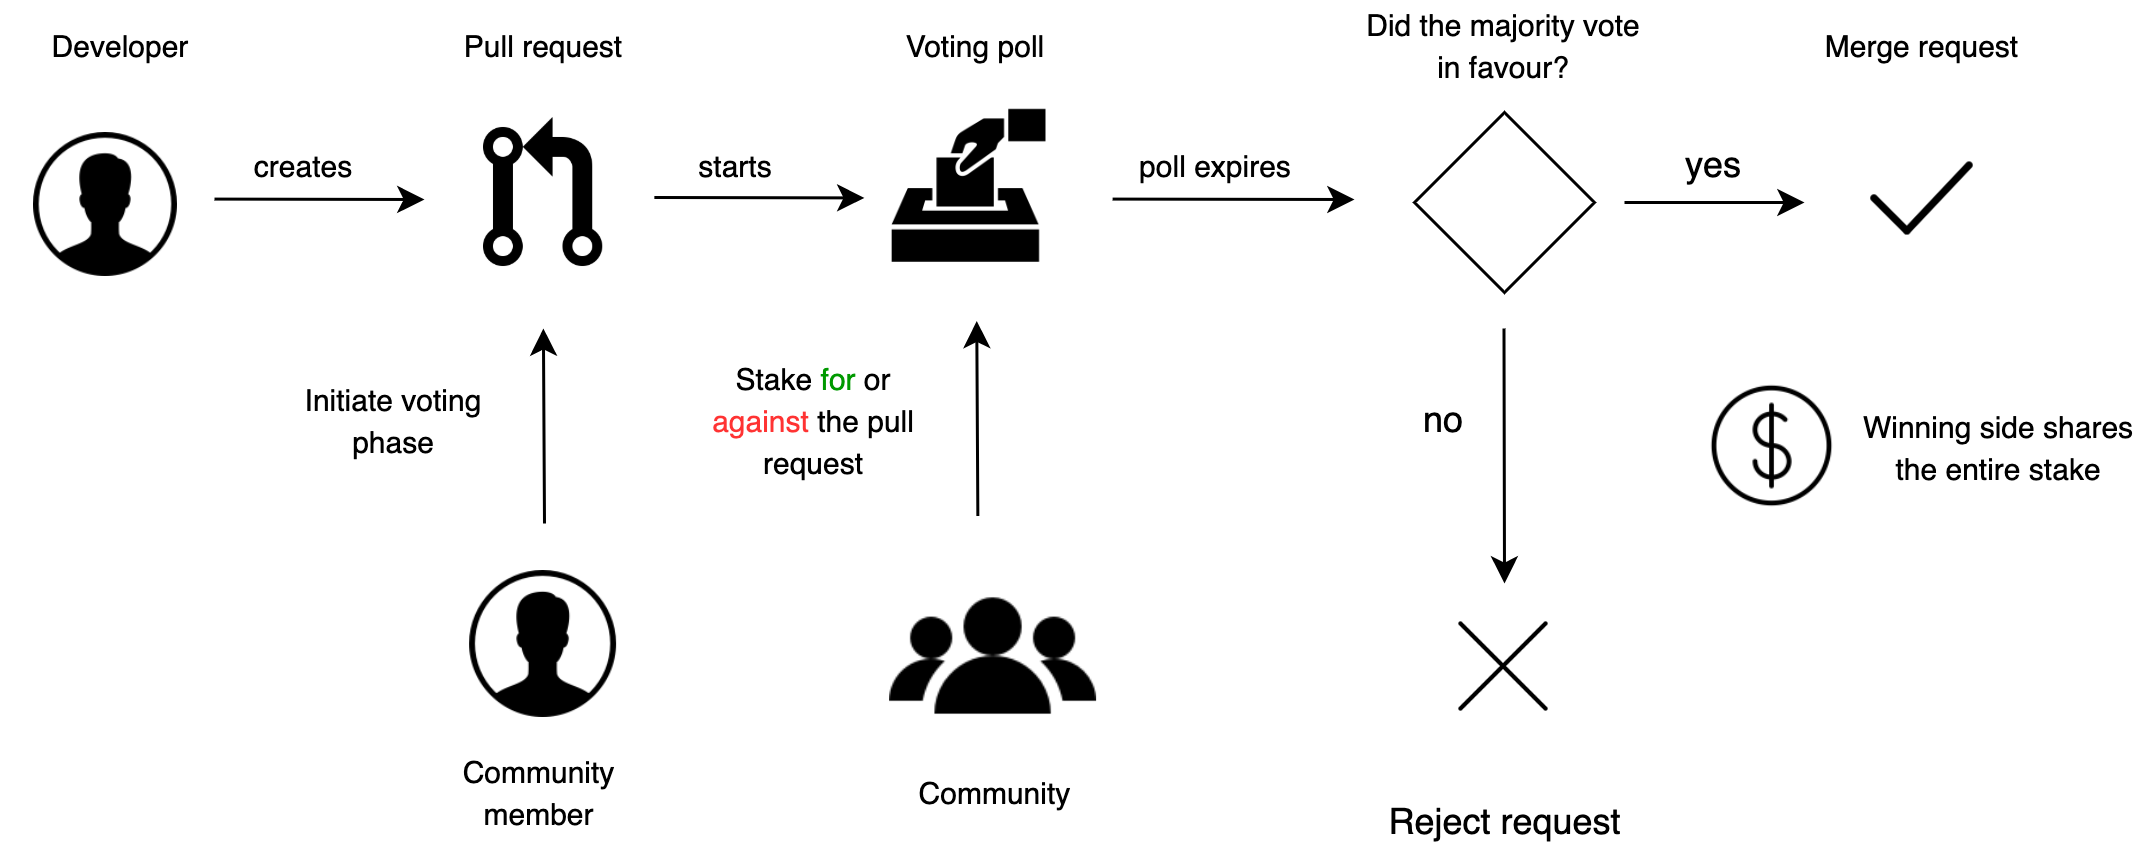
\includegraphics[width=140mm]{images/firstprotocol.png}
	\caption{First version of the extension protocol}
	\label{fig:arch-firstprotocol}
\end{figure*}

\subsection{Second protocol}
As already described, the second protocol is an extension of the first protocol. The decision why we have expanded the first 
protocol is explained in the \textit{5. Discussion}. In general, however, it can be said that we have considered the extension as an 
improvement of the first protocol. The protocol can be basically divided into four phases, which are as follows: \\

\begin{enumerate}
  \item Initialisation and bounty funding
  \item Issue claiming and solution
  \item Pull request voting
  \item Evaluation and distribution \\
\end{enumerate}
During the first phase, the smart contract is created after the initialisation of the bounty process. With the help of this smart contract, 
all further processes such as crowdfunding the bounty, claiming the issue, voting on the pull request and distributing the rewards and 
stakes are orgranised persistent, decentralised and trustless via the Ethereum blockchain. The details of the mentioned processes and 
the individual phases are explained in this section. \\ \\
\textbf{Phase 1: Initialisation and bounty funding} \\
The protocol workflow first starts independently when a community member creates an issue, in the GitHub repository, 
related to a problem or a new feature. If the owner or an authorized user of the open source repository thinks that the issue 
is reasonable, they can initiate a bounty process for the issue. The community can then fund the bounty with their own Ether
 to motivate a developer to solve the issue. A developer can potentially receive this bounty as a reward  if he solves the 
issue in a pull request and the community accepts it. The Ether paid into the bounty is held in a smart contract for a certain 
period of time, so that the bounty cannot be negatively manipulated in the short term. If no developer wants to solve this issue
and the period described above has expired, the the community members that funded the bounty receive their shares back.
(GRAFIK) \\ \\
\textbf{Phase 2: Issue claiming and solution} \\
While the community collects the bounty, a developer can always decide for himself whether the bounty is high enough for him to 
solve the issue. As soon as the reward is high enough that a developer would solve the issue for this amount, he can claim the
issue for him. But the following must be given. No other developer has already reserved the issue, an issue can only be processed 
by one developer. The developer has to pay a collateral to claim the issue, which he can lose if he either does not submit 
a solution within a given period of time or if it is rejected by the community. Once the issue is reserved by a developer, 
he has a certain period of time in which he has to program a solution and provide it as a pull request. If the developer does not 
provide a solution or it is rejected by the community, he loses his stake, which is then sent to the bounty. The issue is then set back 
to the claiming phase. (GRAFIK)\\ \\
\textbf{Phase 3: Pull request voting} \\
This process is the same as the first variant of the protocol, the only differences are that the voting process starts, when 
the developer submits his pull requests and that the staker must include a comment on his 
vote as to why he voted the way he did. This comment is then posted in the comment section of the pull request. \\ \\
\textbf{Phase 4: Evaluation and distribution} \\
As with the first protocol, the minority stakes are transferred to the majority stakers after the voting phase. The difference 
here is that if the pull request is accepted by the community, the developer receives a fixed percentage share of the minority
stakes and the remaining share goes to the majority staker. He also receives the collected bounty and his collateral. However, 
if the pull request is rejected,the developer loses his however, which gets allocated to the bounty and the protocol puts the issue 
back into the claiming phase.

\section{Implementation}
The implementation of the chrome browser extension consists of a frontend and the in \textit{3. Protocol} described protocol.
In this section, the technical implementation of the two components will be explained.Furthermore, for information purposes, 
when the protocol is discussed, the second version of the protocol is meant.
The mentioned chrome extension frontend has been created according to the current standard with HTML, CSS, JavaScript 
and the Chrome extension API \cite{chrome2021api}. In summary, the chrome extension was developed as a kind of web application 
with a few specific limitations. On the other hand, the development and implementation of the protocol required much more thought.
The protocol must connect the Ethereum blockchain with GitHub and, so to speak, mediate the data between the two endpoints. \\ \\
The collaboration with the Ethereum blockchain was done using the JavaScript library web3js \cite{web32021js}. 
This library enables interactions with an 
Ethereum node and thus with the blockchain using HTTP. This allows the chrome extension to retrieve general information from the 
blockchain, but also to write data and even create smart contracts. Querying blockchain data does not require any special settings, 
as it is a read-only request. All write actions on the blockchain, such as voting on a pull request or generating a smart contract, require
 a wallet in the extension, as you have to pay transaction fees for the actions. \\ \\
No special library is needed for the GitHub connection, this is done via the API provided by GitHub \cite{git2021api}. 
This can also be accessed using 
HTTP, which is needed to fetch information about repositories, to create voting comments or to merge or reject a pull request.
In contrast to working with the Ethereum blockchain and smart contracts, many of the requests against the GitHub API require an 
authentication token, which can be fetched via the GitHub oAuth API \cite{git2021auth}. The GitHub oAuth is used as a login in the extension, which
 means that the extension does not need its own login and can therefore fetch the authentication token. However, the token alone 
is not sufficient as authentication for every request; for merging and rejecting pull requests, a developer token must also be stored 
in the extension, which can be obtained from the GitHub account settings. \\ \\
Probably the most difficult aspect of the implementation of the chrome extension is the completion of the voting, i.e. \textit{Phase 4: 
Evaluation and distribution}. Contrary to the other phases and actions, this process must happen automatically as soon as the 
voting phase ends. However, since we only have a client-side programme, we can only detect this when one of the developed 
chrome extensions is running. For this reason, after the GitHub oAuth login, the extension checks if there are completed pull 
request votes and if so, the extension triggers the described workflow \textit{Phase 4: Evaluation and distribution} for the 
pull request in the background.

\section{Discussion}
\textbf{Protocol change}\\
In the course of implementing the first protocol, we found some major flaws in it, which is why we have modified and extended it as 
described in \textit{3. Protocol}. In a conversation with several software developers, the question came up how to protect the protocol from 
malicious users creating pull requests and releasing them for voting.  For this reason, it was decided that the release for voting cannot take
 place through the general community, as otherwise the danger of such attacks is too great. In the second iteration of the protocol, pull 
requests are released by users with administrator rights by opening the bounty for them. At this point, decentralisation must be reduced 
in order to provide more security. In addition, the idea came up to use the bounty system to create a further incentive for development and maintenance in open source projects, which was not given in the first protocol. This adaptation should lead to a free market for the 
development of features or the solution of issues. This also aims to improve the quality of pull requests, as developers have to put effort 
into their development in order for the pull request to be accepted and for them to receive both their collateral and the bounty. \\ \\
\textbf{Advantages and disadvantages of ethereum}\\
At the time of this research paper, Ethereum is one of the largest blockchain platforms with over one million daily transactions \cite{eth2021scan}.
While Ethereum is constantly being developed and improved due to the size of the community, the main blockchain is not currently 
suitable for this application. Currently, the Ethereum fees for a transaction are around 23.70\$ \cite{eth2021fees}. This means that you have to pay this 
fee for every action, whether voting or contributing to an issue. Unfortunately, this is not sustainable, although future developments 
of the Ethereum protocol may change this. Currently, this problem is being avoided by working on the Ethereum testnet Sokol. 
However, this cannot be used in live operation because the Ether on this chain has no value. \\ \\
\textbf{Synchronisation of voting results}\\
The current browser extension approach has the advantage that everything is started from the extension and you can react to misbehaviour 
on the part of the web3js library or GitHub API. However, this approach has difficulties especially when completing voting polls.
Because there is no central server that carries out these changes, there is always the danger that two clients simultaneously initiate 
this process in the background. Although no direct damage can be done, unnecessary transaction fees may be incurre. In addition, it is 
problematic that if a voting phase expires but no one starts the extension for a longer period of time, the associated pull request is not 
merged or rejected and the stakes and bounties are not sent. Also, this implementation requires that community members are willing to 
load their own wallets with Ethereum and pay transaction fees for the actions.

\section{Conclusion and future work}
The presented implementation of the chrome browser extension and the underlying protocol forms a solid basis for a new kind of 
open source development via GitHub. With the help of new technologies such as the blockchain, new possibilities are now available 
for setting up centralised software in a more decentralised and thus also more democratic way. As described above, we see some 
problems with the current implementation and there is also the question of how open the open source community is to this approach. \\ \\
For these reasons, we see two aspects that need to be explored in future work. The first aspect would be a qualitative study of how 
open source developers and community members feel about a decentralised development approach and what they think about such
 things as blockchain and transaction fees. The second aspect would be to investigate whether a server-client architecture is more 
suitable for this application, as was done in the work \textit{Development of a blockchain based access control protocol for 
GitHub repositories} \cite{ulrich2020dev} as Open-Source project. One possibility would be to adapt the server to the requirements
of the browser extension and connect the extension to it. This could be investigated to see if this approach leads to better reliability 
and solves some of our described weaknesses.

%%
%% The next two lines define the bibliography style to be used, and
%% the bibliography file.
\bibliographystyle{ACM-Reference-Format}
\bibliography{sample-base}

%%
%% If your work has an appendix, this is the place to put it.
\appendix

\end{document}
\endinput
%%
%% End of file `sample-sigconf.tex'.
